\chapter{Related Work}

\section{Ad-hoc methods}
	Simple distortion methods are applied to the image privacy protection field such as pixelation and blurring. The pixelation method subsamples the image and the blurring method smoothes images with some filters like Gaussian filter or average filter ~\cite{Agrawal09,Boyle00}. Both by destorying the original image information, pixelation and blurring make a trade between privacy information and image quality. Although these two methods are widely used in practical situations like TV interviews, they suffer from the same risk proposed in ~\cite{Newton05} called parrot attack. General face recognition algorithms figure out the identity by computing the similarity between the target image and database images. Blur and pixelation destory the target image information so that the target image is not similar to any image in database. Parrot attack would preprocess all the database images with pixelation or blurring, then applies face recognition algorithms to pixelated or blurred images so that target images and database images are preprocessed with the similar procedures. 

	\par
	Two more de-identificaiton methods are introduced in ~\cite{Winkler14}: blanking and encryption. The intuitive blanking method in face de-identificaiton is to cut the face region off and replace the region with black color. It also could be extended to paint the region of interest, like face, with background images  ~\cite{inpaint09,Qureshi09}. Compared with other de-identification methods introduced before, encryption has the advantage in recovery ~\cite{Boult05}. With a proper key, the encrypted image is always available to be decrypted so that the image remains useful even if it is covered by a snowboard. These two methods cover image information including both identity and facial expressions. It is the balance between privacy and data utilization that should be the key point in face de-identification. Protecting the identity privacy while preserving facial expressions simultanously is the purpose of our research. 
	
	\par
	Dufaux ~\cite{dufaux08} introduced a privacy protection method using in video sequence by scrambling the locations of pixels in a rectangle range. By controling the range size, different degrees of fuzzy results could be produced. It is possible to recover the original image information if the scrambling order is recorded. Essentially, the scrambling method is a kind of encryption with the permutation order as the encryption key. Scrambling method overcomes other traditional encryption methods in original information preserving. If the scrambling range is in proper size, the original information is still understandable. In another word, scrambling also trades privacy protection with data utility. The images shown in Figure \ref{adhoc_example} retriving from ~\cite{dufaux08} illustrate the examples of different de-identification methods above. 
	% whether place four images here
	\begin{figure}[!htb]
		  \centering
		  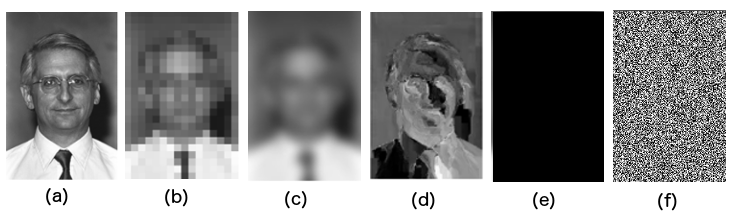
\includegraphics[width=0.9\textwidth]{figure/adhoc.png} 
		  \caption{(a) the origianl image; (b) Pixelation; (c) blurring; (d) scrambling; (e) blanking; (f) encryption}
		  \label{adhoc_example}
	\end{figure}

	\par
	There are still some interesting and simple methods in face de-identification field such as cartooning and face swapping. Converting a real image into cartooning one is a developed technology. Erdélyi ~\cite{erdely14} applied this technology in de-identification area by applying edge detector and mean-shift algorithm in the real image so that the pixels with similar colors would be assign the same value. It is intuitive that cartooning method is able to thwart automatic face recognition algorithms. However, it is hardly deceive a human. Face swapping is also a popular and simple method to de-identify face images. The simplest explanation of this idea is to replace one person's face with another one's. The research in ~\cite{CAVE08} shows the face swapping result could be photorealistic. As a improved version of face swapping method, S. Mosaddegh etc. ~\cite{Mosa14} composes a new face to replace the original one by taking several donors' face parts, thus making the synthetic face contain several persons' characters. 

	\par
	As a summation, the previous de-identification methods are all trade-offs between privacy protection and data utility preservation. When processed by the previous introduced methods, the original face image information would be damaged to protect identity but also erase some data utility such as expressions, gender. In another word, the previous introduced methods protect identity privacy information by destorying all the original image information, which definitely destory the data utility simultaneously. 

\section{K-anonymity based methods}
	K-anonymity is a model proposed by ~\cite{Sweeney02} for privacy protection by 

	\par
	K-same-Pixel

	\par
	K-same-Eign

	\par
	K-same-Model

	\par
	K-same-Select
	
	General solutions model face shape and appearance separately. 